% Příklad použití šablony FM TUL 
% vytvořil Jan Koprnický
% upraveno 14. 1. 2015

% Nastavení šablony
% Nastaven� �ablony FM TUL
% nastaveni prezentace
%\documentclass[draft]{beamer}
\documentclass[t]{beamer}

\usepackage[czech]{babel}

% FONTY

%\usepackage[cp1250]{inputenc} % pro win1250
%\usepackage[T1]{fontenc}

\usepackage[utf8]{inputenc}
\usepackage[IL2]{fontenc}

\usepackage{lmodern}

% XeLaTeX
%\usepackage{fontspec,lipsum}
%\defaultfontfeatures{Ligatures=TeX}
%\usepackage[small,sf,bf]{titlesec}
% 
%\setromanfont{Georgia}
%\setsansfont{Myriad Pro} %Tahoma}
%\setsansfont{Tahoma}
%\setsansfont{Arial}
%\setsansfont{Times New Roman}
%====

% bohu�el dal�� fonty nejsou pln� po�e�t�n�, tedy nejde bez obt�� kop�rovat z PDF

%\usepackage{times}
% \usepackage{avant}
% \usepackage{bookman}
% \usepackage{helvet}  %chyb� tu�n� �ez u strojov�ho p�sma
% \usepackage{newcent}
% \usepackage{palatino} 



%\usepackage[scaled]{uarial}
%\usepackage{helvet}


\usepackage{hyperref}

\mode<presentation>
{
  \definecolor{FM_TUL}{cmyk}{0,0.6,1,0}
  
  \useinnertheme{rectangles}
  
  % VN�J�� BAREVN� T�MA NADPIS�    
  \usecolortheme{whale}  
  
  % VNIT�N� BAREVN� T�MA V��T�, BLOK� ATD.  
  \usecolortheme{orchid}

  \setbeamercolor{titlelike}{parent=structure}
  \setbeamercolor{frametitle}{fg=black}
  \setbeamercolor{title}{fg=black}
  \setbeamercolor{item}{fg=FM_TUL} 
  \setbeamertemplate{navigation symbols}{} % potla�en� naviga�n�ch symbol�
  \setbeamercolor{block title}{fg=white,bg=FM_TUL} % p�edefinov�n� barvy z�kl. bloku
  \setbeamercolor{caption name}{fg=FM_TUL}
  
%  Nadpisy slid� tu�n� dokud nevy�e��m pou�it� font� tak, aby se dalo kop�rovat z pdf
%  \setbeamercolor{frametitle}{fg=FM_TUL}
  \setbeamertemplate{frametitle}
  {
    \textbf{\insertframetitle}
    \par
  }
  \setbeamercolor{bibliography entry author}{fg=black} % literatura �ern� a ne mod�e
  \setbeamercolor{bibliography entry title}{fg=black} % literatura �ern� a ne mod�e
  \setbeamercolor{bibliography entry journal}{fg=black} % literatura �ern� a ne mod�e
  \setbeamercolor{bibliography entry note}{fg=black} % literatura �ern� a ne mod�e
  
%Nefunguje  \setbeamercolor{tableofcontents}{fg=TUL_FM} % obsah TUL_FM a ne mod�e
}

%===============================================================================
% TITULN� STRANA
%===============================================================================
\setbeamertemplate{title page}{
\begin{flushleft}
   
\includegraphics[width=0.6\textwidth]{obr/logo-fm-cmyk-cz.pdf}
\end{flushleft} 
  %
\begin{center} 
  \setbeamercolor{postit}{fg=black,bg=FM_TUL}
%  \begin{beamercolorbox}[center,sep=2pt,wd=\textwidth,ht=3cm,dp=20pt]{postit}
 \begin{beamercolorbox}[center,sep=10pt,wd=\textwidth,ht=3.2cm,ignorebg]{postit}
            
      {\bf {\LARGE \inserttitle}}\\[16pt]
              
      \insertsubtitle
  \end{beamercolorbox}
%
  \vspace{10pt}
  {\bf \small \insertauthor {\color{FM_TUL}}}
%  \vspace{10pt}    
\end{center}
%
\vfill
\vskip0pt plus 1filll
{\color{FM_TUL} \hrule} 
%
\begin{center}
\vspace{-8pt}         
\TextTitulniStranaPodLinkou
\end{center}   
}
%===============================================================================
% Z�HLAV� KA�D�HO SLAJDU
%===============================================================================
\setbeamertemplate{headline}{
  \hspace{-3pt}
\includegraphics[width=0.3\textwidth]{obr/logo-fm-cmyk-cz.pdf}
}
%===============================================================================
\setbeamertemplate{footline}{

\includegraphics[width=\textwidth]{obr/FM_TUL_linka_piktogram_obd.pdf}

\vspace{-9.5pt}
~\hfill {\tiny\color{white} \insertframenumber\,/\,\inserttotalframenumber}\hspace{5pt}

\hspace{3pt} {\tiny \inserttitle {\color{FM_TUL} ~|} \insertdate }\hspace{3pt}
\vspace{3pt}
}
%===============================================================================
% �PRAVA BARVY TEXTU V OBSAHU 
%===============================================================================
\setbeamercolor{section in toc}{fg=black}
\setbeamercolor{subsection in toc}{fg=black}
\setbeamercolor{subsubsection in toc}{fg=black}
\setbeamercolor{button}{bg=FM_TUL}

%\definecolor{links}{HTML}{2A1B81}
\hypersetup{colorlinks,linkcolor=,urlcolor=FM_TUL}

\title{Řešení optimalizační úlohy LASSO pomocí proximálních algoritmů}
%
\author{Václav Langr}
% 
\date{\today} %14.\,1.\,2015} % předefinování data
% Textový obsah pod linkou na titulní straně
\newcommand{\TextTitulniStranaPodLinkou}{\tiny
Studentská 2 {\color{FM_TUL} |} 461\,17 Liberec 2 {\color{FM_TUL} |} 
{vaclav.langr@tul.cz} {\color{FM_TUL} |} 
\href{http://www.fm.tul.cz/}{www.fm.tul.cz}}
%===============================================================================
%===============================================================================
\begin{document} 
\section{Uvod}
\begin{frame}[plain]
\titlepage
\end{frame}
%===============================================================================
%===============================================================================
\section{Info}
\begin{frame}
	\vfill
	\begin{block}{Vedoucí práce}
	    doc. Ing. Zbyněk Koldovský, Ph.D.
	\end{block}
	\begin{block}{Cíl práce}
    \begin{itemize}
        \item Nastudovat vlastnosti optimalizační úlohy LASSO
        \item Implementovat proximální algoritmus řešící optimalizační úlohu LASSO v MATLABu
        \item Vytvořit Monte Carlo simulaci a sledovat závislost kvadratické chyby vypočteného signálu od správného řešení na parametru lambda
      \end{itemize}
    \end{block}
\end{frame}
\section{Optimalizační úloha LASSO}
\vfill
\begin{frame}
	\vfill
	\begin{block}{Základní měření signálů}
	$y = A \times x$
	\end{block}
	\begin{block}{Optimalizační úloha LASSO}
		$\underset{x} {\mathrm{argmin}} ~\left\{\left\|y-A \times x\right\| ^2 _2+ \lambda \times \left\|x\right\|_1\right\}$
	\end{block}
\end{frame}
\section{Proximální algoritmus}
\begin{frame}
	\vfill
	\begin{block}{Derivace $\left\| \cdot \right\|_{2}^{2} $}
		$\partial f(x) = -2 \times A^T \times (y-A \times x)$
	\end{block}
			\begin{block}{Proximální algoritmus}
				$x_{n+1} = prox_{\lambda \times step}(x_{n}- step \times \partial f(x_{n}))$
			\end{block}
\end{frame}
\begin{frame}
	\vfill
	\begin{figure}[!ht]
		\begin{center}
			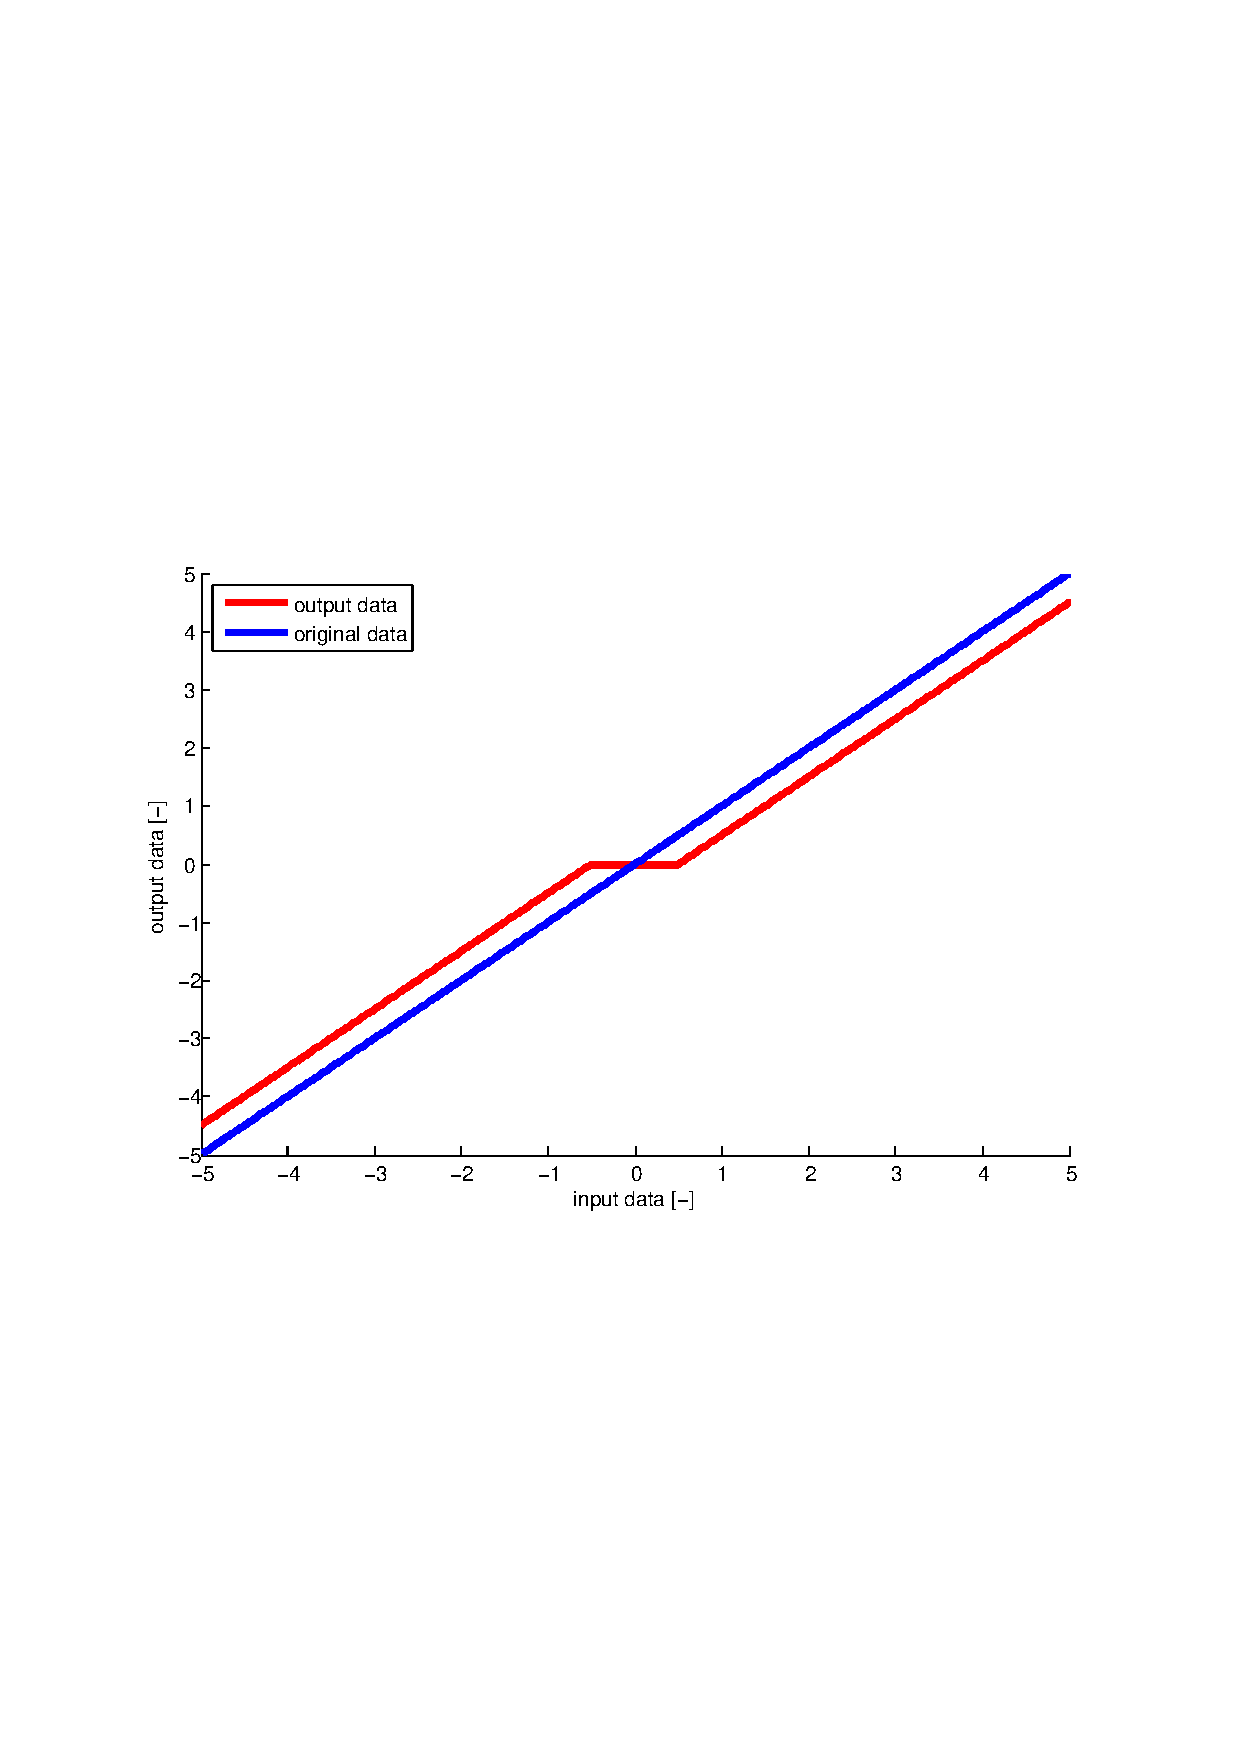
\includegraphics[scale=0.6]{obr/threshhold.pdf}
		\end{center}
		\caption{Průběh měkkého prahování}
		\label{fig:nse}
	\end{figure}
\end{frame}
\section{Video}
\begin{frame}
	\vfill
	\begin{center}
		{\Large \bfseries
			Ukázka průběhu proximálního algoritmu
		} 
	\end{center}
\end{frame}
\section{Monte Carlo simulace}
\begin{frame}
	\vfill
	\begin{block}{Monte Carlo simulace}
		\begin{itemize}
			\item Jednoduché na implementaci
			\item Na sobě nezávislá data
			\item Odpovídající výsledky
		\end{itemize}
	\end{block}
\end{frame}
\begin{frame}
	\vfill
	\begin{figure}[!ht]
		\begin{center}
			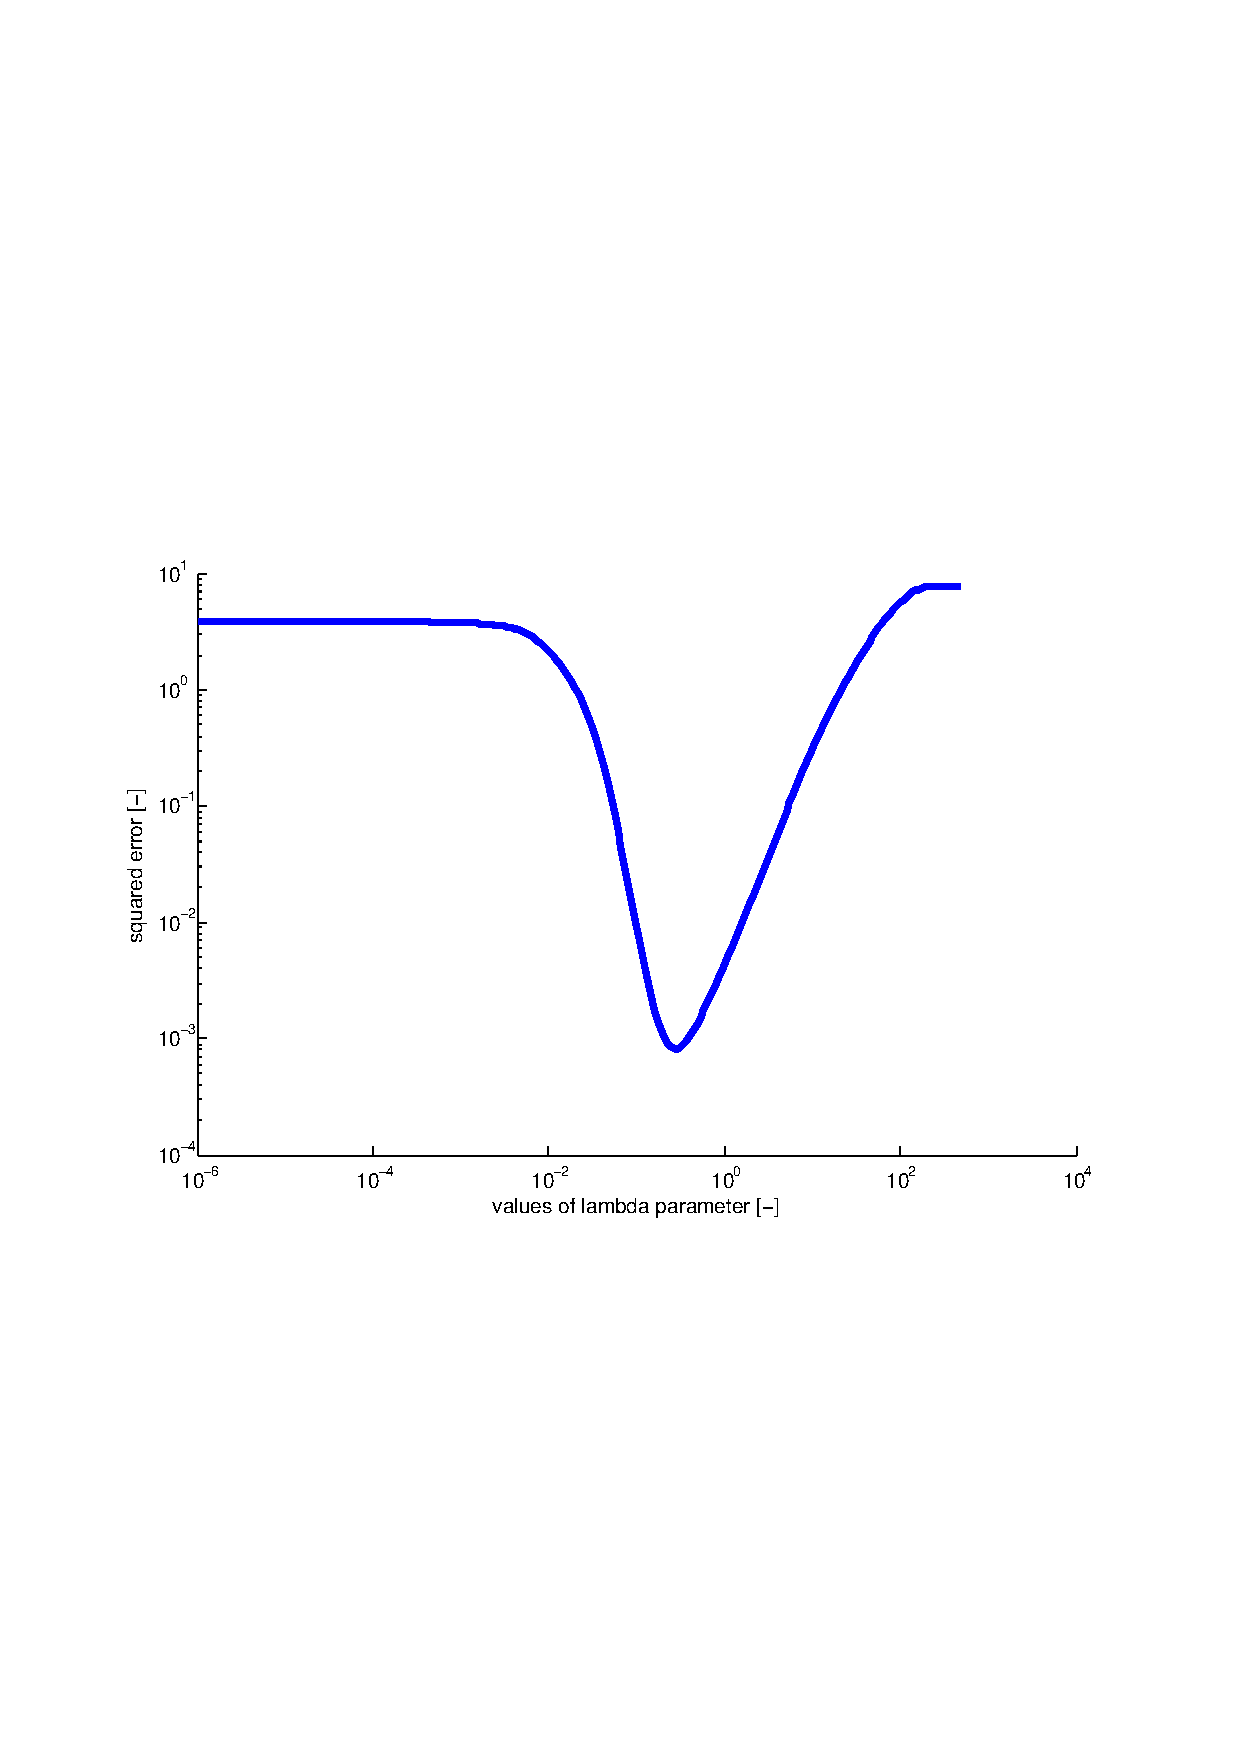
\includegraphics[scale=0.6]{obr/nse.pdf}
		\end{center}
		\caption{Kvadratická chyba nalezeného řešení a původních dat}
		\label{fig:nse}
	\end{figure}
\end{frame}
\begin{frame}
	\vfill
	\begin{block}{Analytická předpověď}
		\begin{itemize}
			\item Obtížné pro $l_{2}^{2}$ LASSO
			\item Využívá se $l_{2}$ LASSO spolu s mapovací funkcí
		\end{itemize}
	\end{block}
\end{frame}
\begin{frame}
	\vfill
		\begin{figure}[!ht]
			\begin{center}
				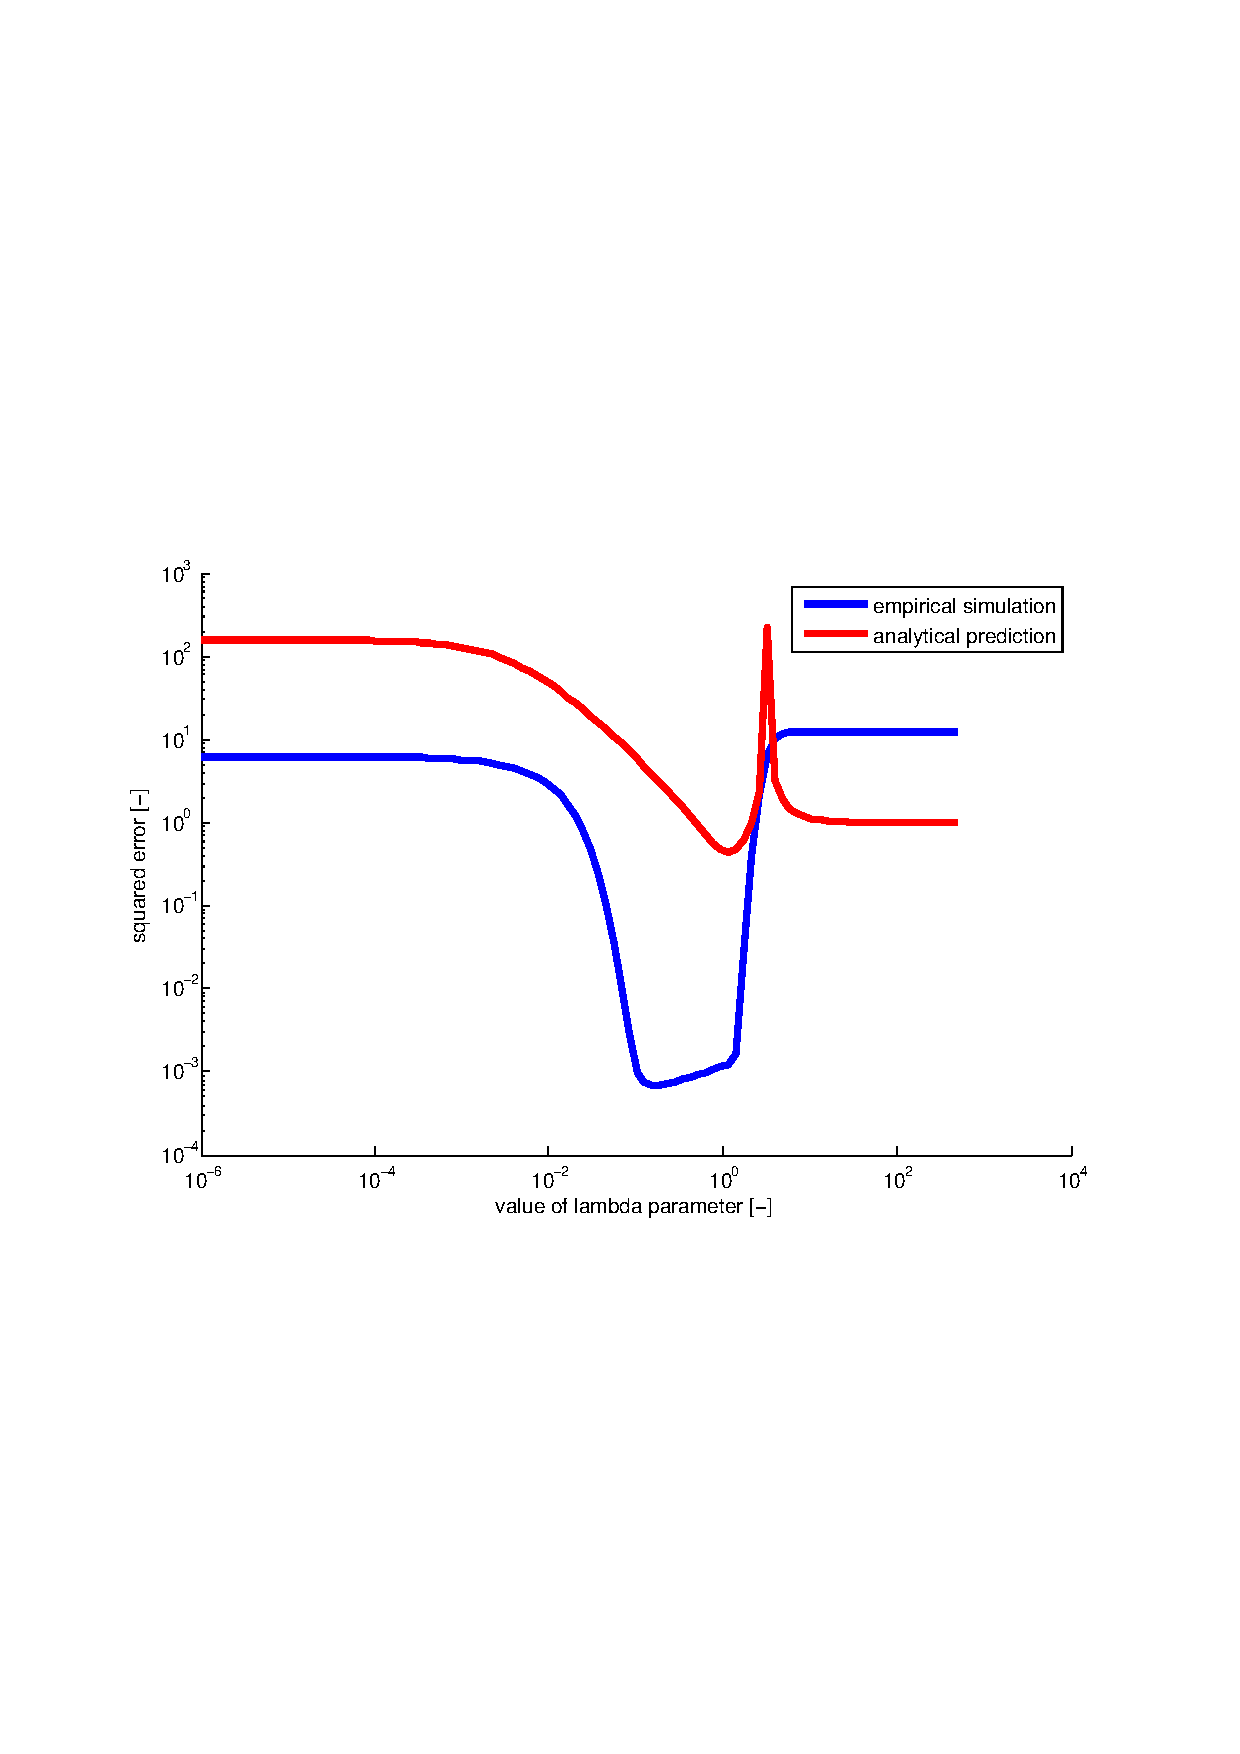
\includegraphics[scale=0.55]{obr/nsel2.pdf}
			\end{center}
			\caption{Porovnání analytické předpovědi a kvadratické chyby empirického pozorování}
			\label{fig:nsel2}
		\end{figure}
\end{frame}
%===============================================================================
\section{Podekovani}
\begin{frame}
	\vfill
  \begin{center}
  {\Large \bfseries
    Děkuji za pozornost.
    } 
  \end{center}
  
  \begin{center}
  	{\Large \bfseries
  		Prostor pro otázky.
  	} 
  \end{center}
\end{frame}
\end{document}
